%
%  outline latex source document for AV assignment 1.
%  use pdflatex to format this.
%
\documentclass[10pt,a4paper,oneclumn]{article}
\usepackage{amssymb,amsmath}            % if some maths is needed
\usepackage{graphicx}                   % if any images are to be included
% pick a different font if desired
\usepackage{times}

\title{Advanced Vision Assignment 2 Report}  % AILP: please use this title.
\author{Mindaugas Dabulskis, Marat Subkhankulov}                      % replace with name or exam number
\date{26th February 2013}                 % replace with actual date

\begin{document}

\maketitle  % insert title, author info
%
\section{Introduction}

This report describes the work carried out for the second assignment of the AV course.
The aim of the assignment was to track three coloured balls through a set of video frames.
The algorithm for ball detection and segmentation is discussed. 
The performance of the approach is evaluated using a gold standard.

\section{Algorithm and implementation}

In order to segment out the balls from the subject image (the current frame being considered), we removed background regions, and thresholded using values obtained from training data.

The following regions had to be removed from the image: 
\begin{enumerate}
\item Static background
\item Juggler's clothing
\item Juggler's hands
\item Juggler's face
\item Shadow caused by the juggler on the door
\end{enumerate}

To remove the above regions the following techniques were applied:

\begin{enumerate}
\item Mask 1: Average background subtraction
\item Mask 2: Clothing mask based on intensity
\item Mask 3: Hand skin mask based on saturation
\item Classification based on a training sample
\end{enumerate}

\begin{figure}
\centering
  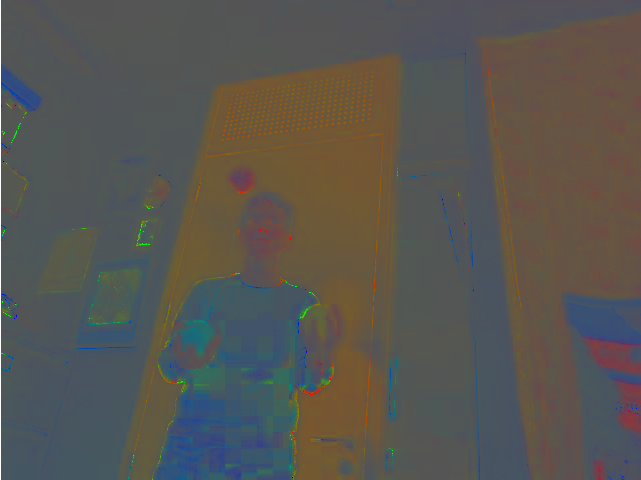
\includegraphics[width=6cm]{figures/imnrgb.png}
  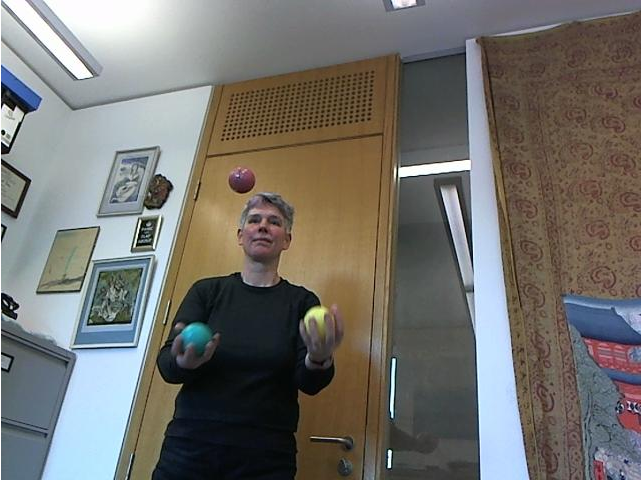
\includegraphics[width=6cm]{figures/original.png}
\caption{Training sample for each ball}
\end{figure}

\subsection{Mask 1: Average background}

A picture of the empty room had been given, however when subtraction of the background from the subject image did not eliminate the shadow of the door, which had similar values to the yellow ball even in normalized RGB. Thus we obtained a mean of all the frames and used the resulting image as the background; By converting the subject and the new background images to N-RGB, subtracting and thresholding out the low brightness regions we obtained a mask which eliminated:
\begin{enumerate}
\item Static background
\item Shadow on the door
\item Juggler's face
\end{enumerate}

\begin{figure}
\centering
  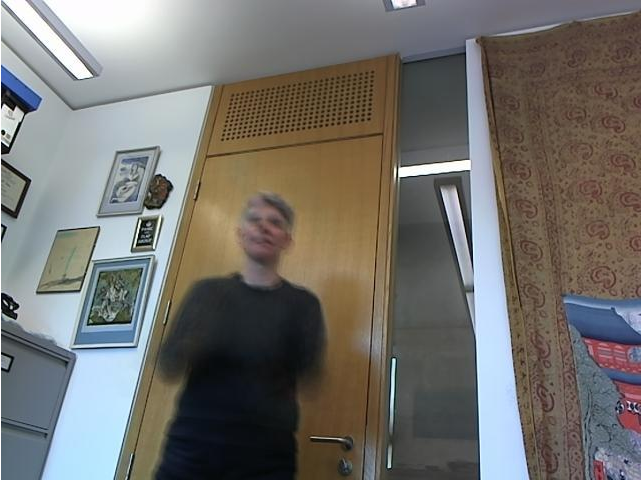
\includegraphics[width=3cm]{figures/av.png}
  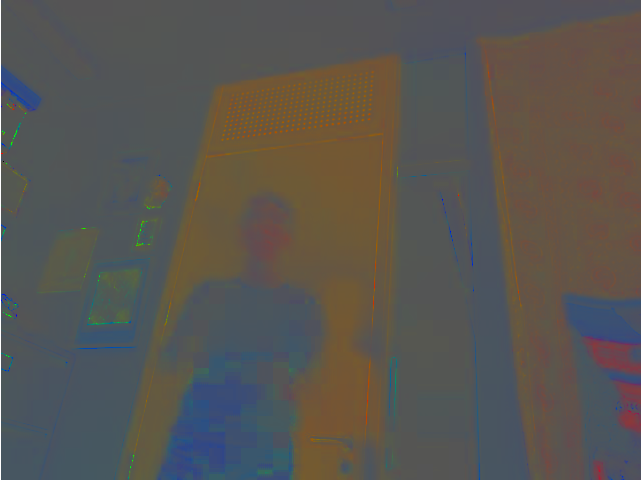
\includegraphics[width=3cm]{figures/avnrgb.png}
  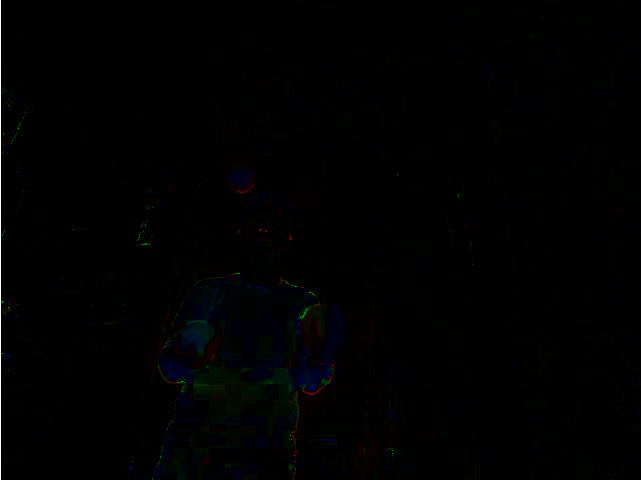
\includegraphics[width=3cm]{figures/avnrgbdif.png}
  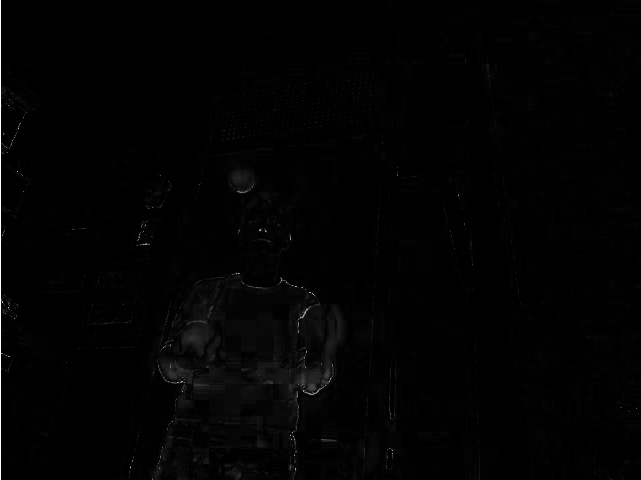
\includegraphics[width=3cm]{figures/avnrgbhsvvalue.png}
  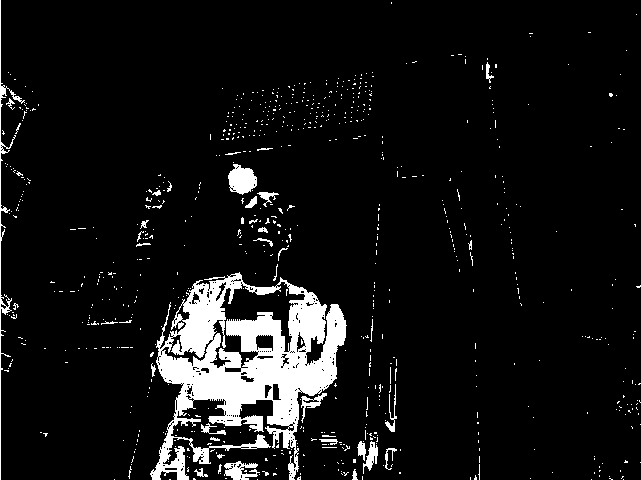
\includegraphics[width=3cm]{figures/avnrgbdifhsvmask.png}
\caption{Training sample for each ball}
\end{figure}

\subsection{Mask 2: Clothing mask}

Mask 1 did not remove the clothing of the juggler due to the smoothing effect of averaging; This posed a problem as the clothes had similar chromaticity to the green ball. We took advantage of the clothes' dark colour to easily theshold out the clothing using a manual threshold.

\begin{figure}
\centering
  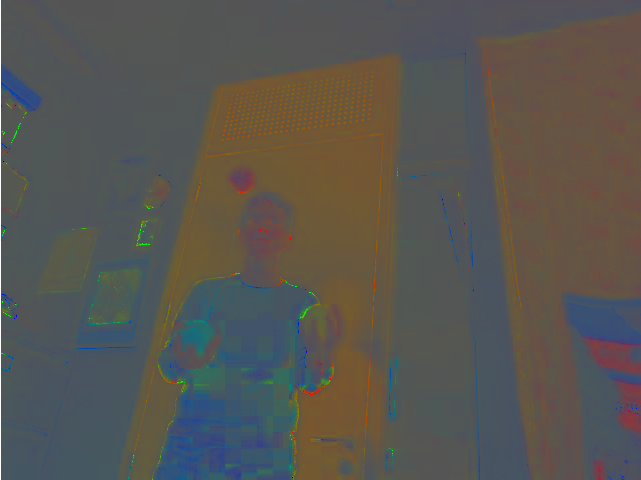
\includegraphics[width=3cm]{figures/imnrgb.png}
  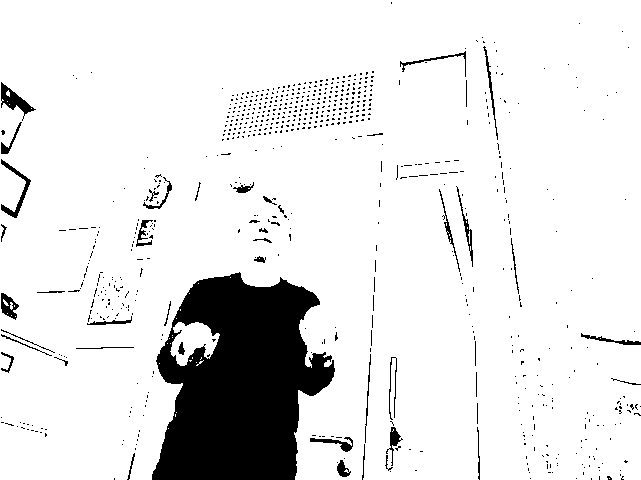
\includegraphics[width=3cm]{figures/clothes_mask.png}
\caption{Training sample for each ball}
\end{figure}

\subsection{Mask 3: Hands}
It seemed reasonable to use N-RGB for segmenting out the balls as the lighting effects were lare largely removed, however the hands of the juggler were not removed by the previous masks and had similar chromaticity to the red ball. We removed the hands by taking advantage of the skin's unique saturation value.

\begin{figure}
\centering
  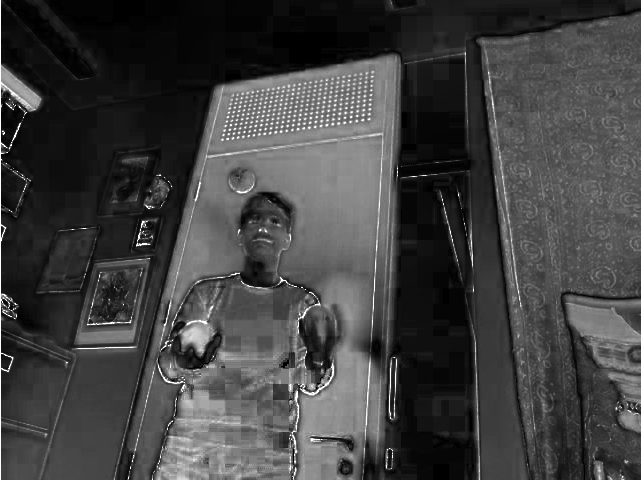
\includegraphics[width=6cm]{figures/imsat.png}
  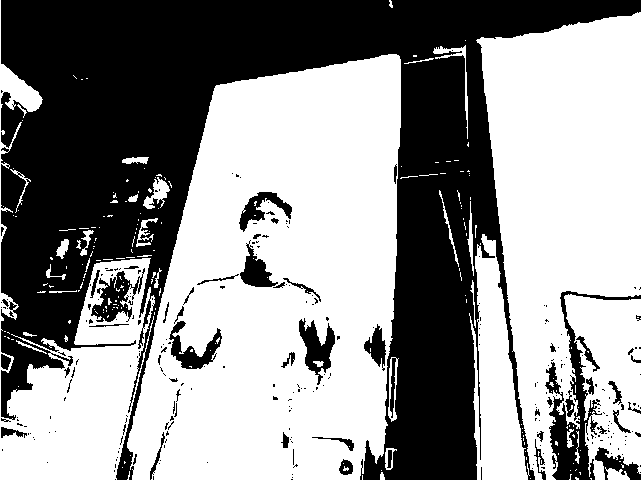
\includegraphics[width=6cm]{figures/imhsvsatmask.png}
\caption{Training sample for each ball}
\end{figure}

\subsection{Segmentation}

Having applied all of the masks the background was largely removed. Thresholding could now be performed. Conversion to N-RGB eliminated diffuse and specular lighting effects on the balls, but necessitated thresholding on all three channels; Since the intensity of all the pixels was largely the same after normalization, it was clear that the majority of variation lies in the hue of the spheres - using this single value simplified thresholding as only one channel could be used to successfully classify the ball pixels. 

\begin{figure}
\centering
  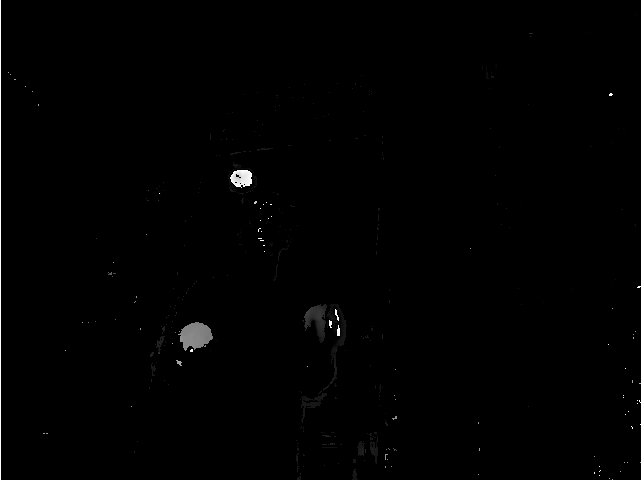
\includegraphics[width=6cm]{figures/bgremoved.png}
\caption{Training sample for each ball}
\end{figure}

Threshold values for hue were obtained from a training sample. The training sample obtained by sampling the pixel as the centroid of each ball given by the ground truth. The lower and upper thresholds were 2 standard deviations from the median of the sample - this was done to ignore outliers.

\begin{figure}
\centering
  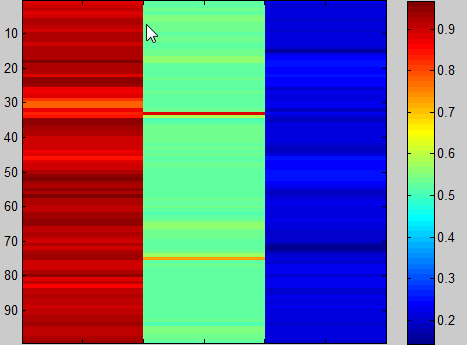
\includegraphics[width=6cm]{figures/training.png}
  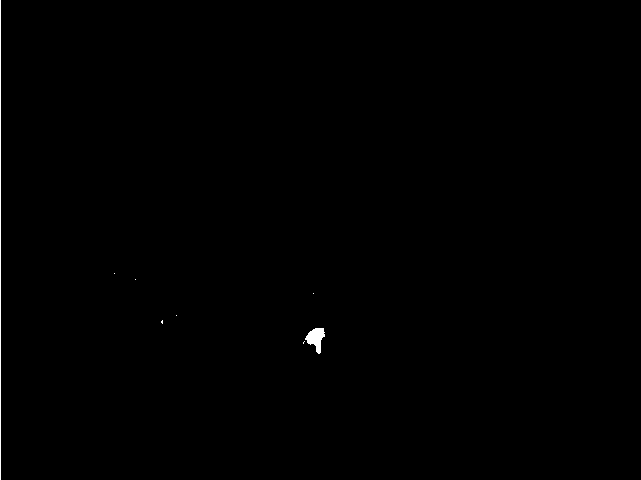
\includegraphics[width=6cm]{figures/class1.png}
  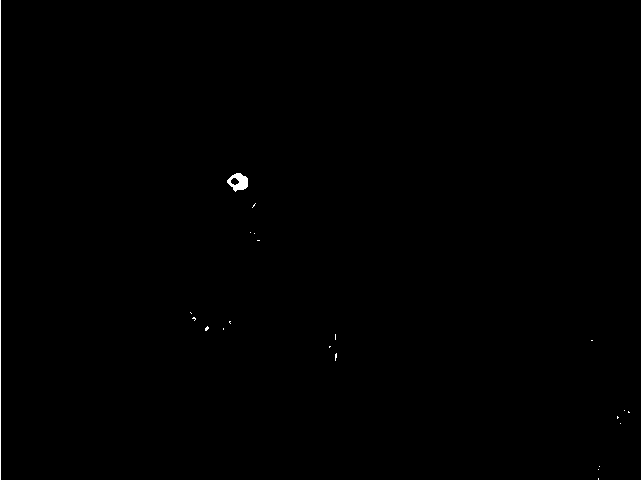
\includegraphics[width=6cm]{figures/class2.png}
  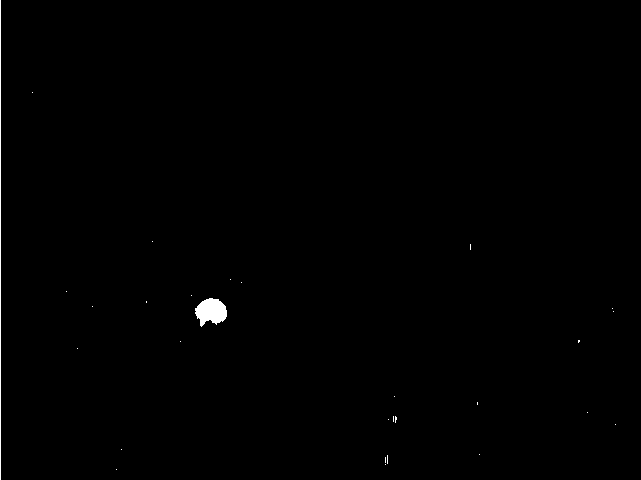
\includegraphics[width=6cm]{figures/class3.png}
\caption{Training sample for each ball}
\end{figure}

\subsection{Clean up}

\begin{figure}[h!]
\centering
  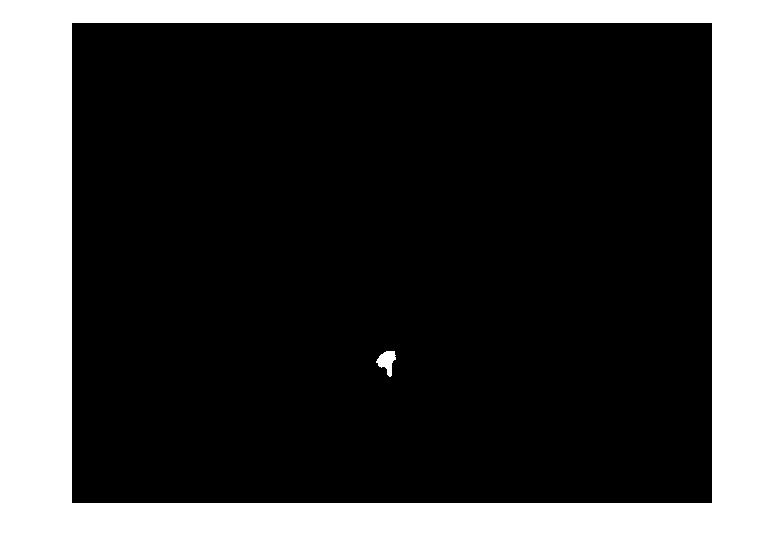
\includegraphics[width=5cm]{cleanedYell.jpg}
  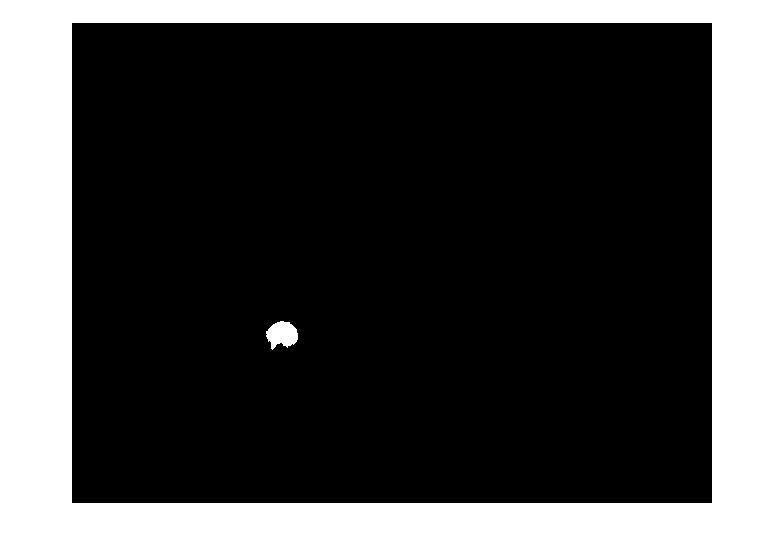
\includegraphics[width=5cm]{cleanGreen.jpg}
  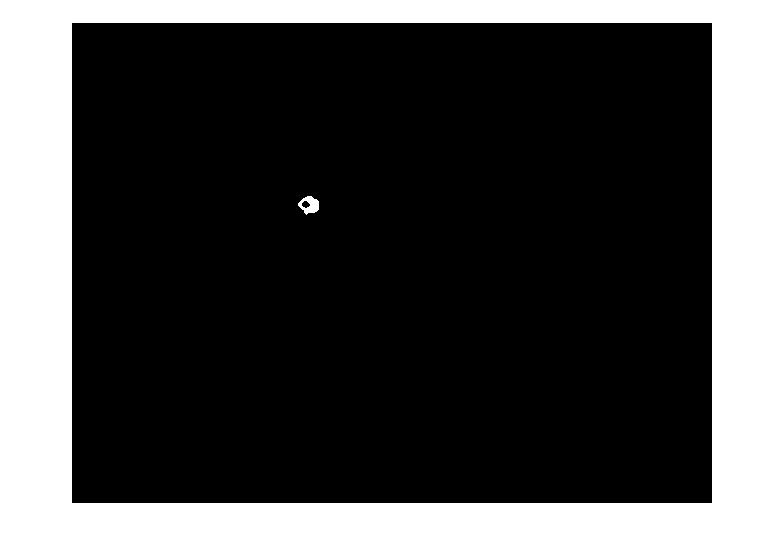
\includegraphics[width=5cm]{cleanRed.jpg}
  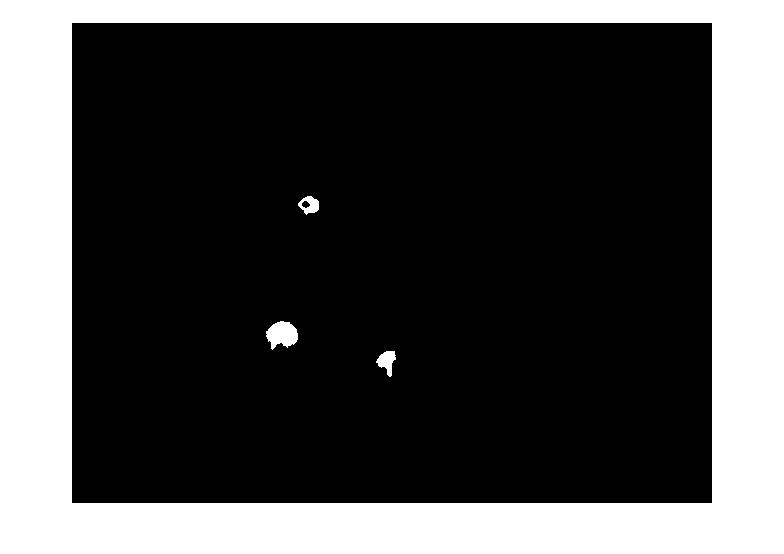
\includegraphics[width=5cm]{cleanAll.jpg}
\caption{Cleaned images}
\end{figure}

Final clean up and ball identification was made using matlab \textbf{bwlabel} and \textbf{regionprops} functions. The function \textbf{bwlabel} takes our intermediate file, which we got after applying all the masks, and labels all the connected objects in the file. Later, this file is supplied to \textbf{regionprops} function, which measures and returns set of the properties for each connected object in the file. We only needed three properties:

\begin{enumerate}
\item \emph{Area} - number of actual pixels in the region,
\item \emph{PixelIdxList} - vector containing the linear indices of the pixels in region,
\item \emph{PixelList} - matrix specifying the locations of pixels in the region.
\end{enumerate}

The idea was: 
\begin{enumerate}
\item to find maximum connected object in the file by the pixels area, 
\item set all other connected object areas pixel to 0 (delete these areas), 
\item find the middle point of the largest connected objects area. 
\end{enumerate}

Second point cleaned the image of all the noise, because the object with biggest area was the ball itself. Third point was needed for evaluation, to evaluate how much our detected ball differs from ground truth. We had four different approaches how to calculate the mass of the ball:

\begin{enumerate}
\item Use the mean of the area pixels,
\item use the median of the area pixels,
\item use the maximum and minimum pixels in \textbf{y} and \textbf{x} coordinates and find the mean between them. This creates a bounding box of the area and finds it centre.
\end{enumerate}

The evaluation of these approaches are reported in the section below. We decided to use just normal mean, but left an option to change if needed and found that other approaches with different data sets works better. We stored all found centres in the matrix. The format of that matrix is exactly the same as the format for the ground truth. In next stage we just plot the found mass centres on each image with the centre from ground truth and draw the trajectory at the end by connecting all the points.


\end{document}
